\documentclass[10pt]{beamer}
\usepackage[utf8]{inputenc}
\usepackage[font=tiny,labelfont=bf]{caption}
\usepackage{dirtytalk}
\DeclareCaptionFont{tiny}{\tiny}
\usepackage{natbib}
\usepackage{subcaption}
%\setbeamersize{text margin left=0.5,text margin right=0.5} 
\usepackage{lipsum}
\usepackage{graphics}
\usepackage[colorlinks=true,linkcolor=blue,citecolor=blue]{hyperref}
\hypersetup{colorlinks,linkcolor=,urlcolor=links}
\newcommand\Wider[2][3em]{%
\makebox[\linewidth][c]{%
  \begin{minipage}{\dimexpr\textwidth+#1\relax}
  \raggedright#2
  \end{minipage}%
  }%
}

\title[Violence amid COVID-19]{Violence Against Women amid COVID-19: The Effects of Social and Traditional Media Campaigns to Empower
Women}
\author[Elizabeth K. Parker-Magyar]{Fotini Christia, Horacio Larreguy, Norhan Muhab \& Elizabeth Parker-Magyar}
\institute[MIT]{Massachusetts Institute of Technology}

\begin{document}

\begin{frame}{}
    \titlepage
\end{frame}

\begin{frame}{Motivation and Question}
\begin{center}
    \begin{itemize}
        \item COVID-19 has heightened the extent and risk of gender-based violence (GBV) and intimate-partner violence (IPV), particularly in the Global South.
%The policies implemented to help contain the spread of COVID-19 have often included significant mobility restrictions. These policies had imposed a significant toll on the economy adding significant economic stress to the existing social stress and reducing women economic empowerment. Combined with existing social norms toward women, these policies ultimately increased the extent and risk of GBV and IPV of women across the globe.
        \vspace{5pt}
        \item Edutainment interventions aimed at empowering women subjected to GBV and IPV have been in person and most successful ones usually have a communal component.
        \vspace{5pt}        
        \item Social distancing and mobility restrictions make these much needed interventions infeasible, and call for alternative ways to disseminate information on risks and services, as well as to offer support.
        \vspace{5pt}        
        \item Surge in the use of social media platforms during COVID-19. 
% Need to add good reference from here https://en.wikipedia.org/wiki/Impact_of_the_COVID-19_pandemic_on_social_media
% https://www.nytimes.com/interactive/2020/04/07/technology/coronavirus-internet-use.html
        \vspace{5pt}        
        \item  \textbf{Question:} Can edutainment interventions delivered through social and traditional media empower women against GBV and IPV?
% Moreover, there is the question of whether previous edutainment interventions requiring substantial resources can be scaled up by exploiting traditional and social media.
    \end{itemize}
\end{center}
    
\end{frame}

%%%%----

\section{Literature}
\begin{frame}{Existing Work}
\begin{itemize}
    %\onslide<1-> 
    \item GBV and IPV are widespread, undermine, economic development, and increase social inequality   \small(Krug 2002). \normalsize
    %\onslide<2-> 
    \item GBV and IPV are highly prevalent in the Global South, especially in the Arab world \small(Hawcroft et. al. (2019), Elghossain et. al. (2019)). \normalsize 
    %\onslide<3-> 
    \item Lack of knowledge of rights and resources and fears of social sanctioning due to existing norms limit women’s willingness to report and seek help (Cooper et al. (2020))
    %\onslide<4-> 
    \item Edutainment interventions posit that exposure to role models' behavior can shift perceptions of social norms, driving changes in attitudes, behaviors, or both  \small(Paluck and Green 2009, Blair et. al 2019). \normalsize
    %\onslide<5-> 
    \item Interventions on  GBV and IPV have had mixed effects:
    \begin{itemize}
        \item Some communally-transmitted interventions increased rejection of violence against women,  \small(Arias 2019, Banerjee et al 2019). \normalisize
         % TV shows but commmucal screening.  
        \item Others find no attitude shift, but increased willingness to report violence \small(Green et. al. 2019, Cooper at. al. 2020).  
    \end{itemize} \normalisize

\end{itemize}
\end{frame}

\section{Context and Intervention}
\begin{frame}{Our Study}
\begin{columns}[T]\begin{column}{0.6\textwidth}
\begin{itemize}
    \onslide<1->\item We partnered with a well-established Egyptian women's rights organization running an ongoing television show. \vspace{2mm}
    \onslide<2->\item We evaluated the impact of their social media and TV programming on: \vspace{2mm}
    \begin{itemize}
        \item Attitudes toward GBV and IPV; \vspace{1mm}
        \item Knowledge and use of resources; \vspace{1mm}
        \item Hypothetical and reported behavior; \vspace{1mm}
        \item Future outlook on gender rights in Egypt
    \end{itemize}
\end{itemize}
\end{column}
\begin{column}{0.5\textwidth}
\begin{figure}\onslide<1->
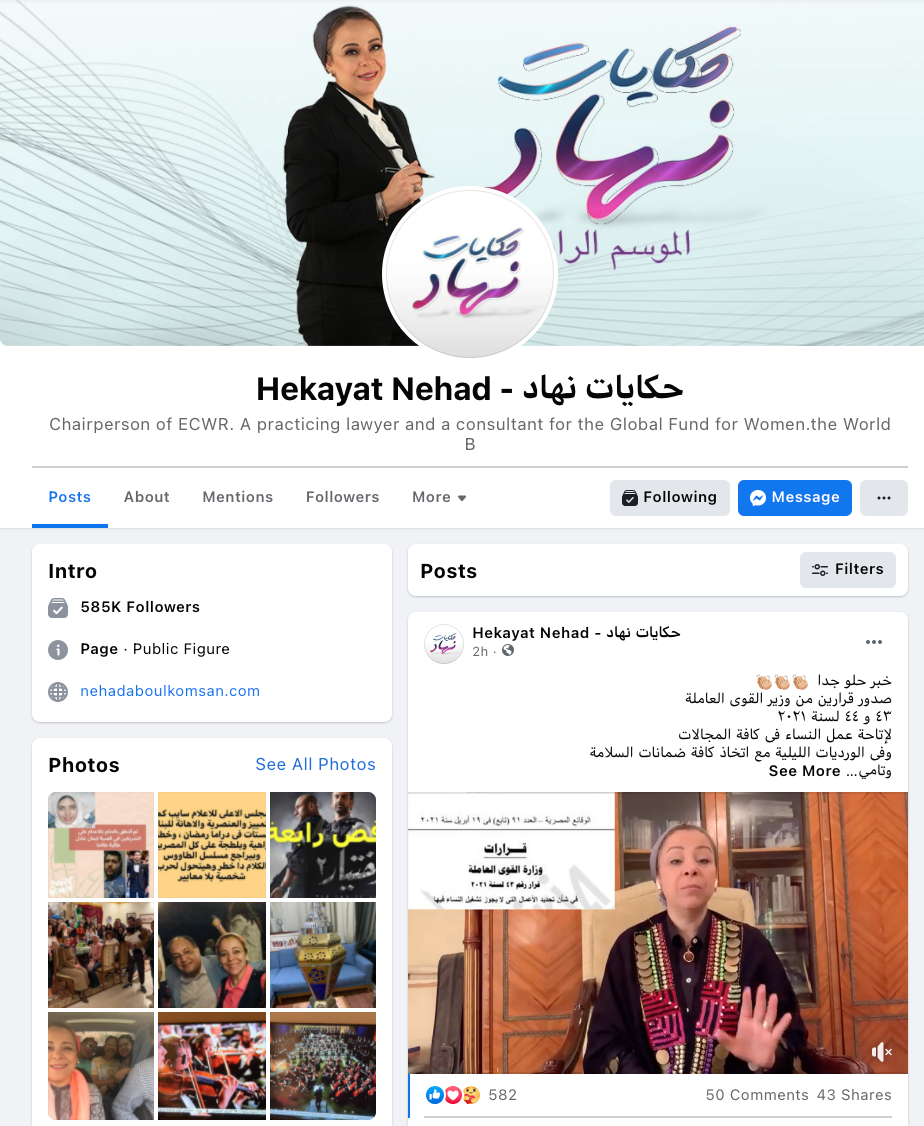
\includegraphics[width = 0.8\textwidth]{Recruit_Intervention/hakayat nehad.png}\captionsetup{font=small, width = 0.9\linewidth}
\caption{\scriptsizeptsize Nehad Abou El Qomsan and the Egyptian Center for Women's Rights have a broad following in Egypt.} \end{figure} 
\end{column}
\end{columns}
\end{frame}

\begin{frame}{Baseline Recruitment via Facebook and Sample}
\begin{itemize}
    \item We used Facebook advertisements to recruit Egyptian women to a baseline survey, with a 25 EGY (1.59 USD) mobile credit incentive.
    \item We surveyed approximately 10,000, of whom 5,828 signed up to receive additional content
\end{itemize}
\begin{figure}
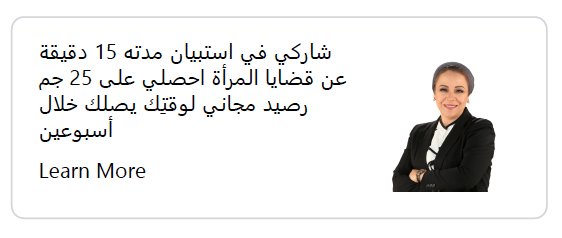
\includegraphics[height = 0.4\textwidth]{Recruit_Intervention/FB_ad_example.png}\captionsetup{font=small, width = 0.9\linewidth}
\caption{\scriptsizeptsize A sample Facebook advertisement featuring our partner and an invitation to a survey about women's issues in Egypt.} \end{figure} 
\end{frame}

% \begin{frame}{Baseline Recruitment via Facebook and Sample}
% \begin{itemize}
%     \item The resulting sample featured broadly similar demographic characteristics as Egyptian female internet users from the 2018 nationally representative Arab Barometer survey.
% \end{itemize}
% \begin{centering}
% \begin{figure}
% 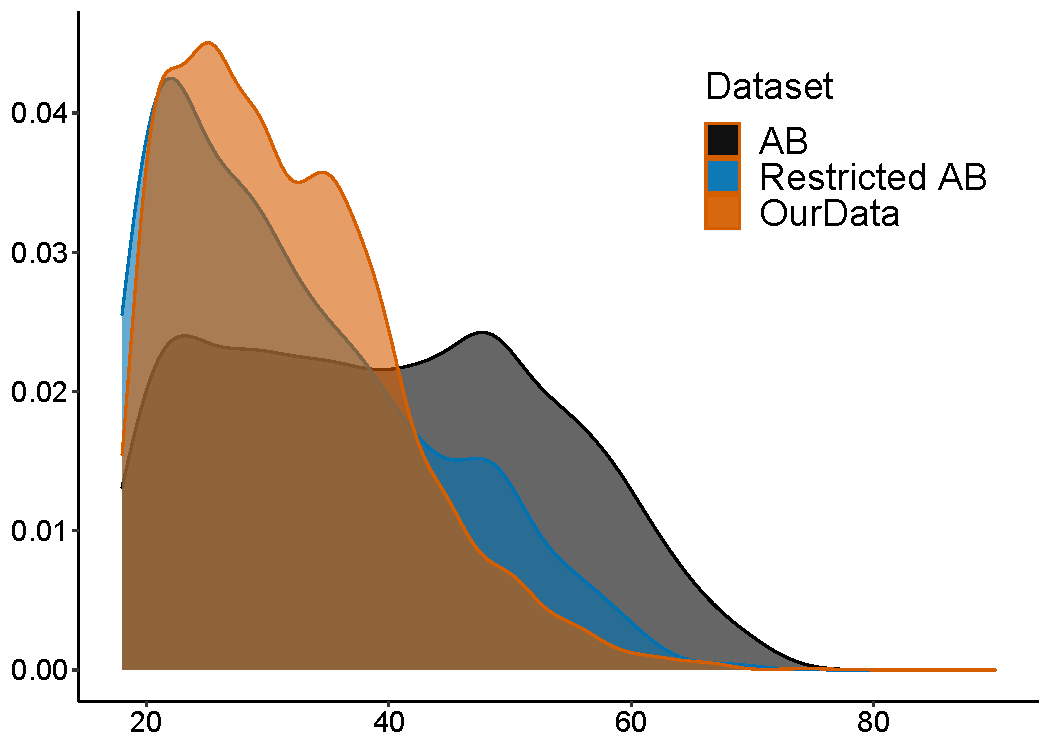
\includegraphics[height = 0.3\textwidth]{Figures/AB/Filled/age.pdf}
% 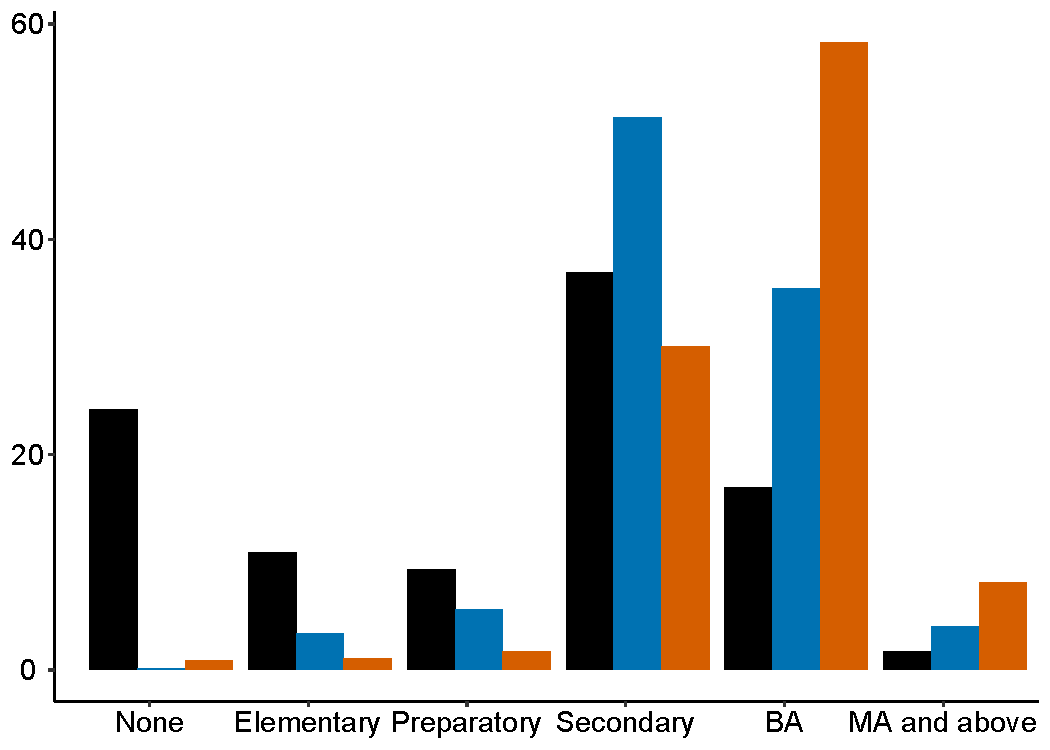
\includegraphics[height = 0.3\textwidth]{Figures/AB/Filled/educ.pdf}
% \captionsetup{font=small}
% \caption{A sample Facebook advertisement featuring our partner and an invitation to a survey about women's issues in Egypt.} \end{figure} 
% \end{centering}
% \end{frame}

\begin{frame}{Sample Demographics Compared with Nationally Representative Arab Barometer}
\Wider[9em]{
\begin{figure}[H]
    \centering
  %  \caption{Comparison of demographics with general (Arab Barometer) population \\}
\begin{subfigure}{0.25\textwidth}
  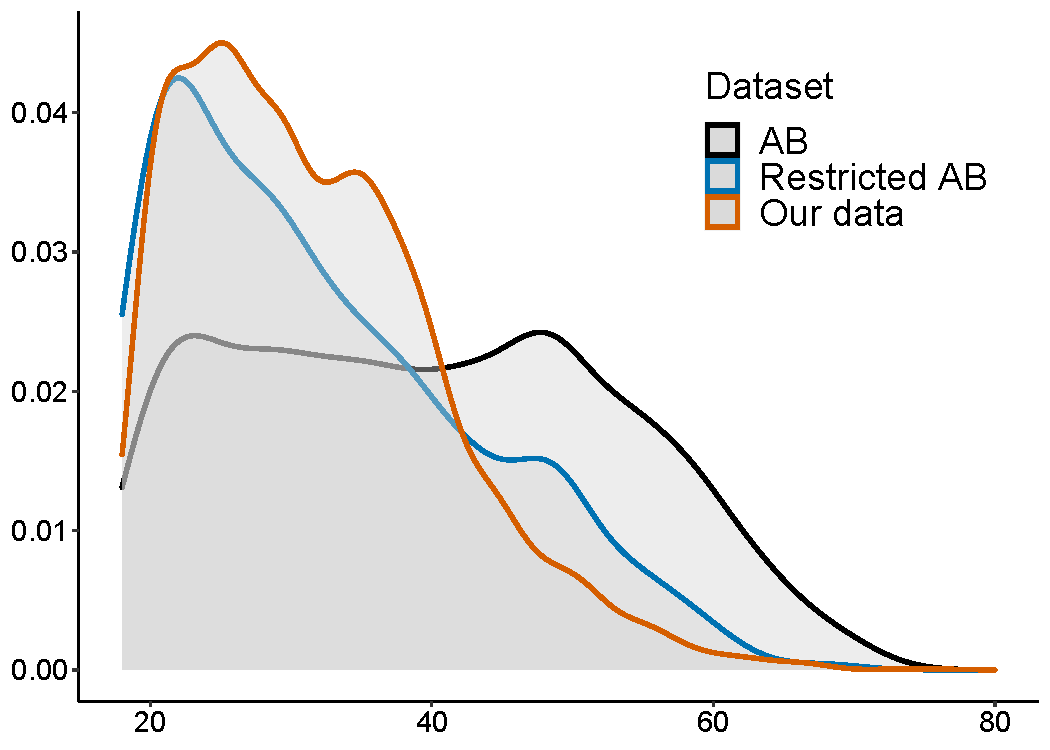
\includegraphics[height=2.9cm,width=4cm\linewidth, clip=true, trim = 0 5 0 5]{Figures/AB/grey_solid/age.pdf}  
    \caption{\scriptsizeptsize Age}
  \label{fig:1}
\end{subfigure}\hfil
\begin{subfigure}{0.25\textwidth}
  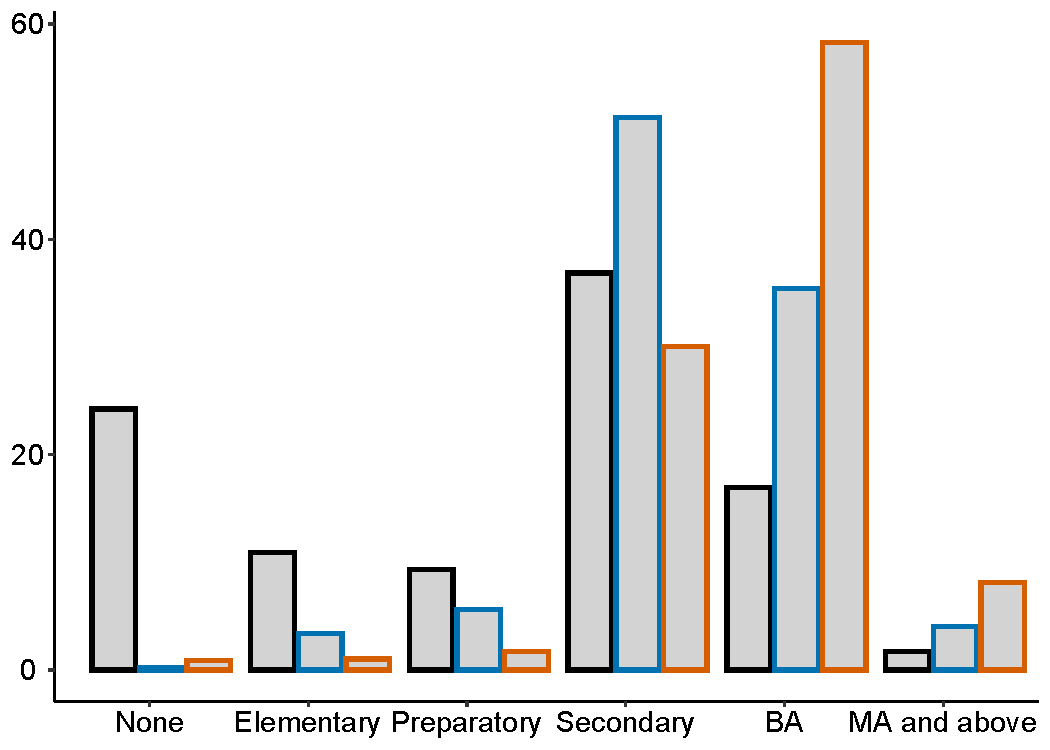
\includegraphics[height=2.9cm,width=4cm\linewidth, clip=true, trim = 0 5 0 5]{Figures/AB/grey_solid/educ.pdf}
    \caption{\scriptsizeptsize Level of education}
  \label{fig:2}
\end{subfigure}\hfil
\begin{subfigure}{0.25\textwidth}
  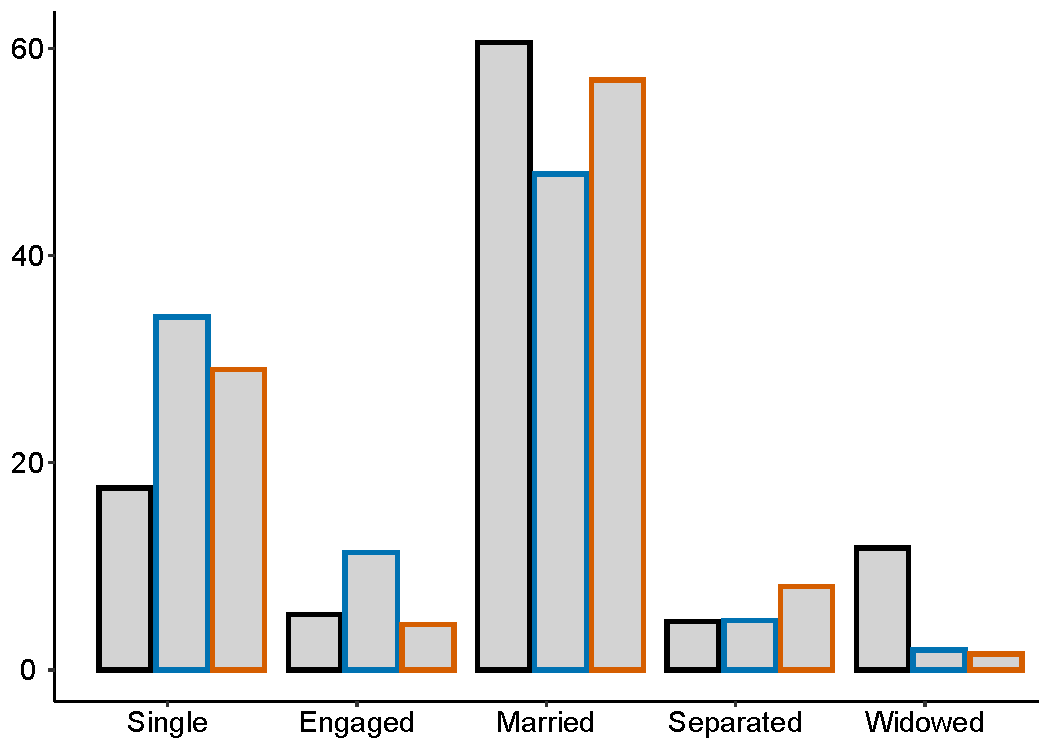
\includegraphics[height=2.9cm,width=3.5cm\linewidth,clip=true, trim = 0 5 0 5]{Figures/AB/grey_solid/married.pdf}
    \caption{\scriptsizeptsize Social status}
  \label{fig:3}
\end{subfigure}
\medskip
\begin{subfigure}{0.25\textwidth}
  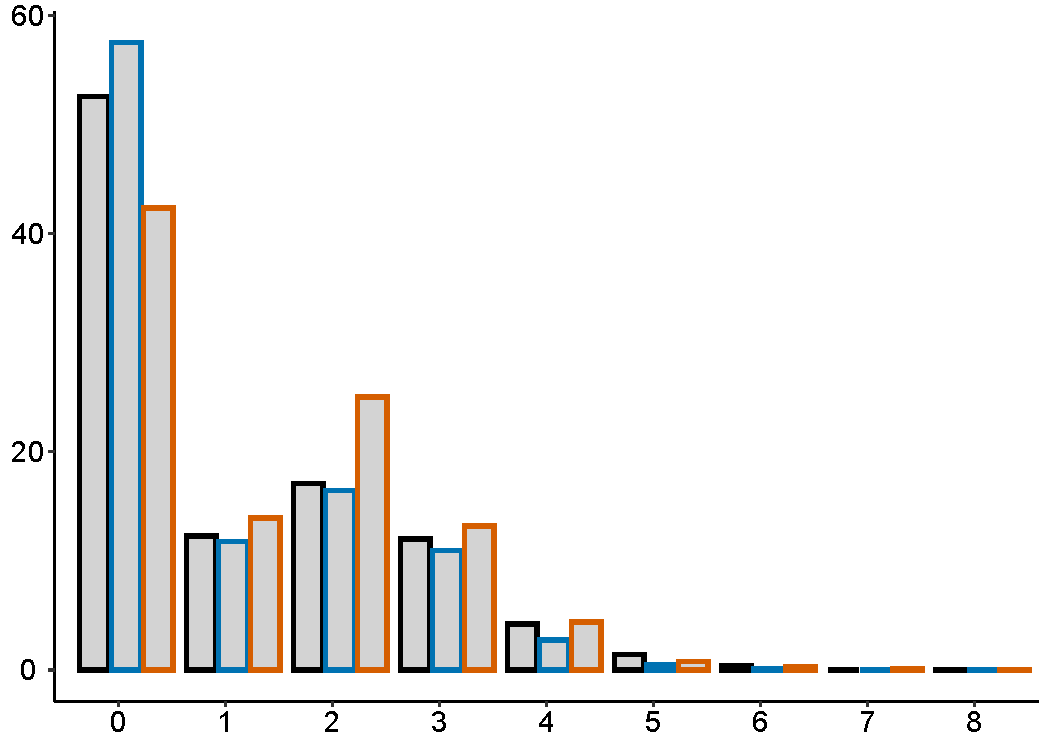
\includegraphics[height=2.9cm,width=4cm\linewidth, clip=true, trim = 0 5 0 5]{Figures/AB/grey_solid/child.pdf}
    \caption{ \scriptsizeptsize Number of children}
  \label{fig:4}
\end{subfigure}\hfil
\begin{subfigure}{0.25\textwidth}
  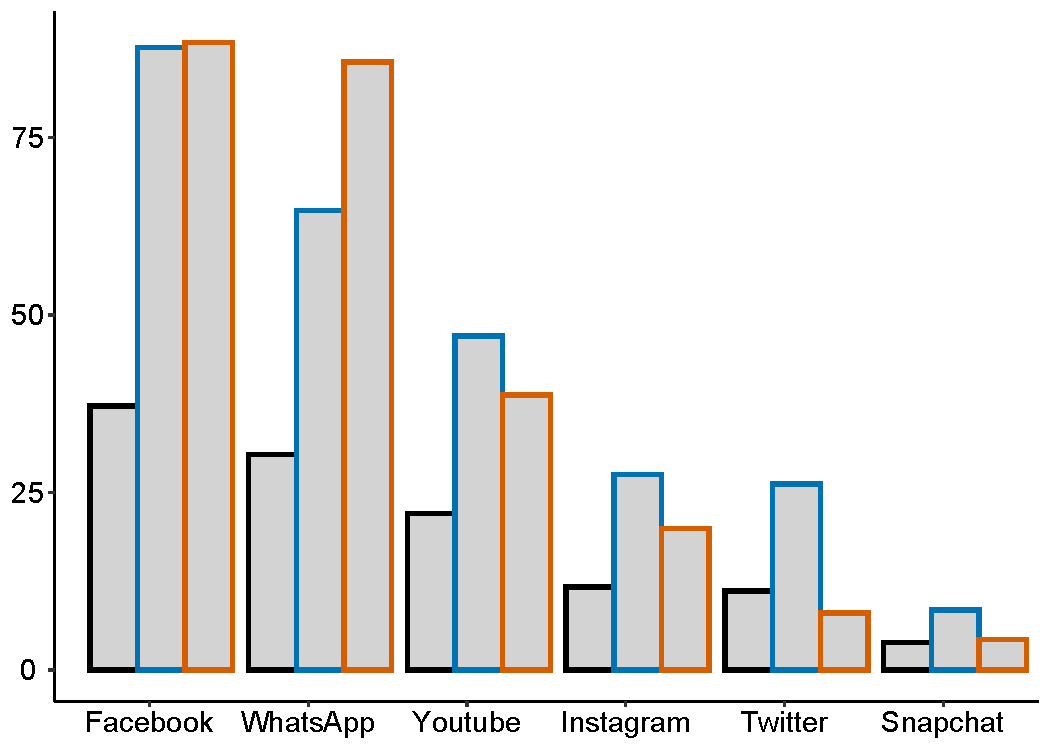
\includegraphics[height=2.9cm,width=4cm\linewidth, clip=true, trim = 0 5 0 5]{Figures/AB/grey_solid/which_sm.pdf}
    \caption{\scriptsizeptsize Social media use}
  \label{fig:5}
\end{subfigure}\hfil
\begin{subfigure}{0.25\textwidth}
  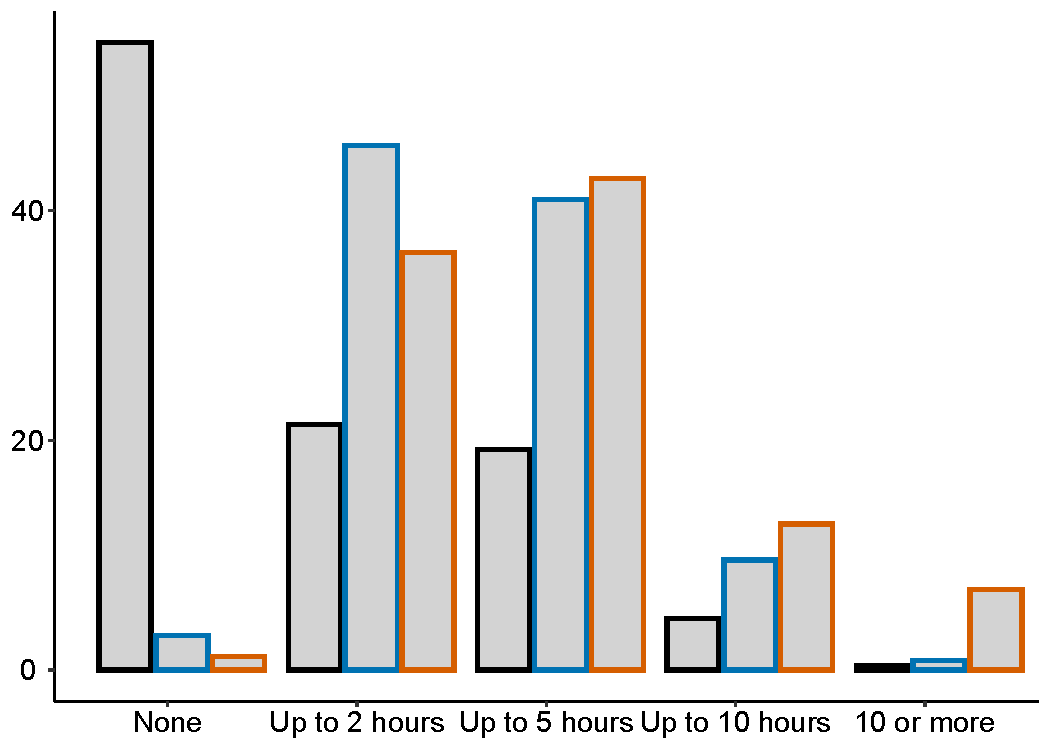
\includegraphics[height=2.9cm,width=3.5cm\linewidth, clip=true, trim = 0 5 0 5]{Figures/AB/grey_solid/hours_sm.pdf}
   % \captionsetup{width=1.5\linewidth}%
    \caption{\scriptsizeptsize Time on social media}
  \label{fig:6}
\end{subfigure}
\end{figure}}
\end{frame}
    

\begin{frame}{Dissemination of Videos and Reminders of Television Show}
\begin{columns}[T] \begin{column}{0.55\textwidth}
\begin{itemize}
    \onslide<1-> \item We enrolled respondents to baseline survey in one of five arms:
    \begin{itemize}
    \onslide<2-> 
    \item 1-3: Messages delivered via WhatsApp (Individually or in Groups) or Facebook with links to a website hosting short videos 
     \onslide<3-> 
    \item 4: A reminder of an ongoing TV show and where it could be viewed
    \onslide<4->
    \item 5: A control group that received links to all content after endline
    \end{itemize}
    \onslide<5-> \item Individuals received messages with links to 13 videos or or 8 TV show reminders and 3 messages with links to previous shows over 8 weeks from July-Sept. 2020
   % \onslide<3-> \item Content focused on diverse issues facing women, centered around violence and harassment.
   % \onslide<4-> \item 75\% balanced endline response rate. 
\end{itemize}
\end{column}
\begin{column}{0.5\textwidth}
\begin{figure}\onslide<1-> 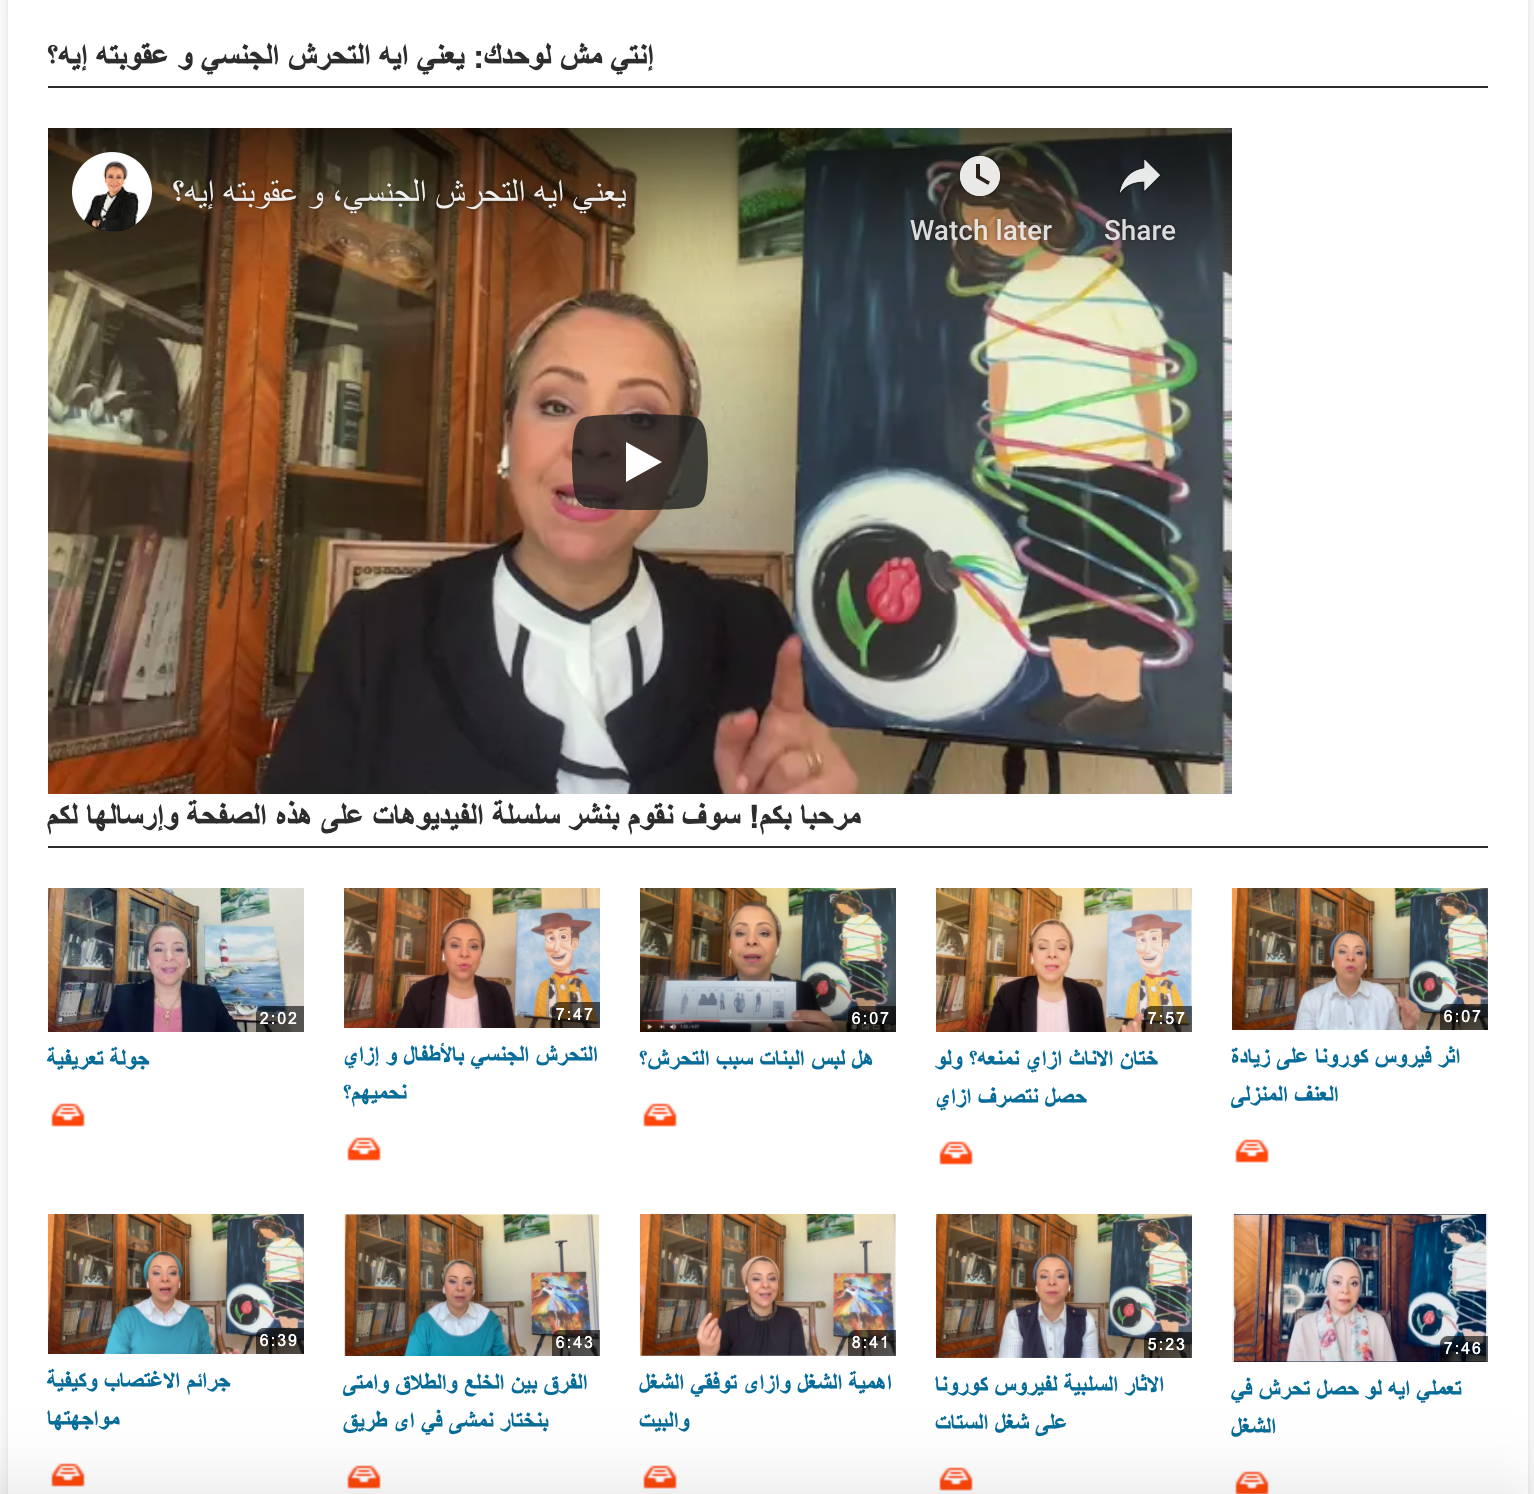
\includegraphics[width = 1\textwidth]{Recruit_Intervention/mshlwa7dek.org:egypt:v1wfb.png}\captionsetup{font=small}
\caption{Participants enrolled in social media treatments received links to a website featuring our partner's video content.} 
\end{figure} 
\end{column}
\end{columns}
\end{frame}

\begin{frame}{Dissemination of Videos and Reminders of Television Show}
\begin{columns}[T] \begin{column}{0.55\textwidth}
\begin{itemize}
    \onslide<1-> \item Content focused on diverse social issues related to gender in Egypt, GBV and IPV:
    \begin{itemize}
        \item Do young women's clothes cause harassment?
        \item What is sexual harassment and what is its penalty?
        \item How can men stand against violence against women?
        \item COVID-19 and domestic violence
    \end{itemize}
    \onslide<2-> \item At endline, response rates were balanced at 75\% across groups. 
\end{itemize}
\end{column}
\begin{column}{0.5\textwidth}
\begin{figure}\onslide<1-> 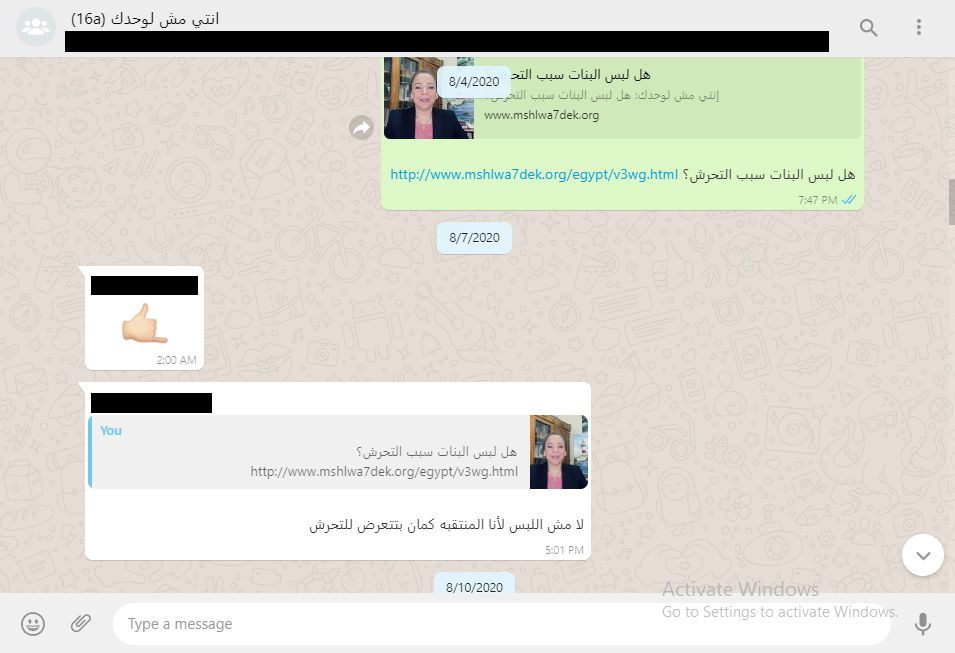
\includegraphics[width = 1\textwidth]{Recruit_Intervention/30.png}\captionsetup{font=small}
\caption{An individual responds over WhatsApp to a video titled, \say{Do women's clothes cause harassment?,} with \say{No, because I wear the niqab and I am also harassed.}} 
 \end{figure} 
\end{column}
\end{columns}
\end{frame}

\begin{frame}{Content of TV Show and Short Videos}
Our partner is a high-status figure who delivered information in an accessible, informal tone similar to edutainment interventions. The set-up differed slightly across TV and social media.
\begin{columns}[T] \begin{column}{0.5\textwidth}
\begin{figure}\onslide<1-> 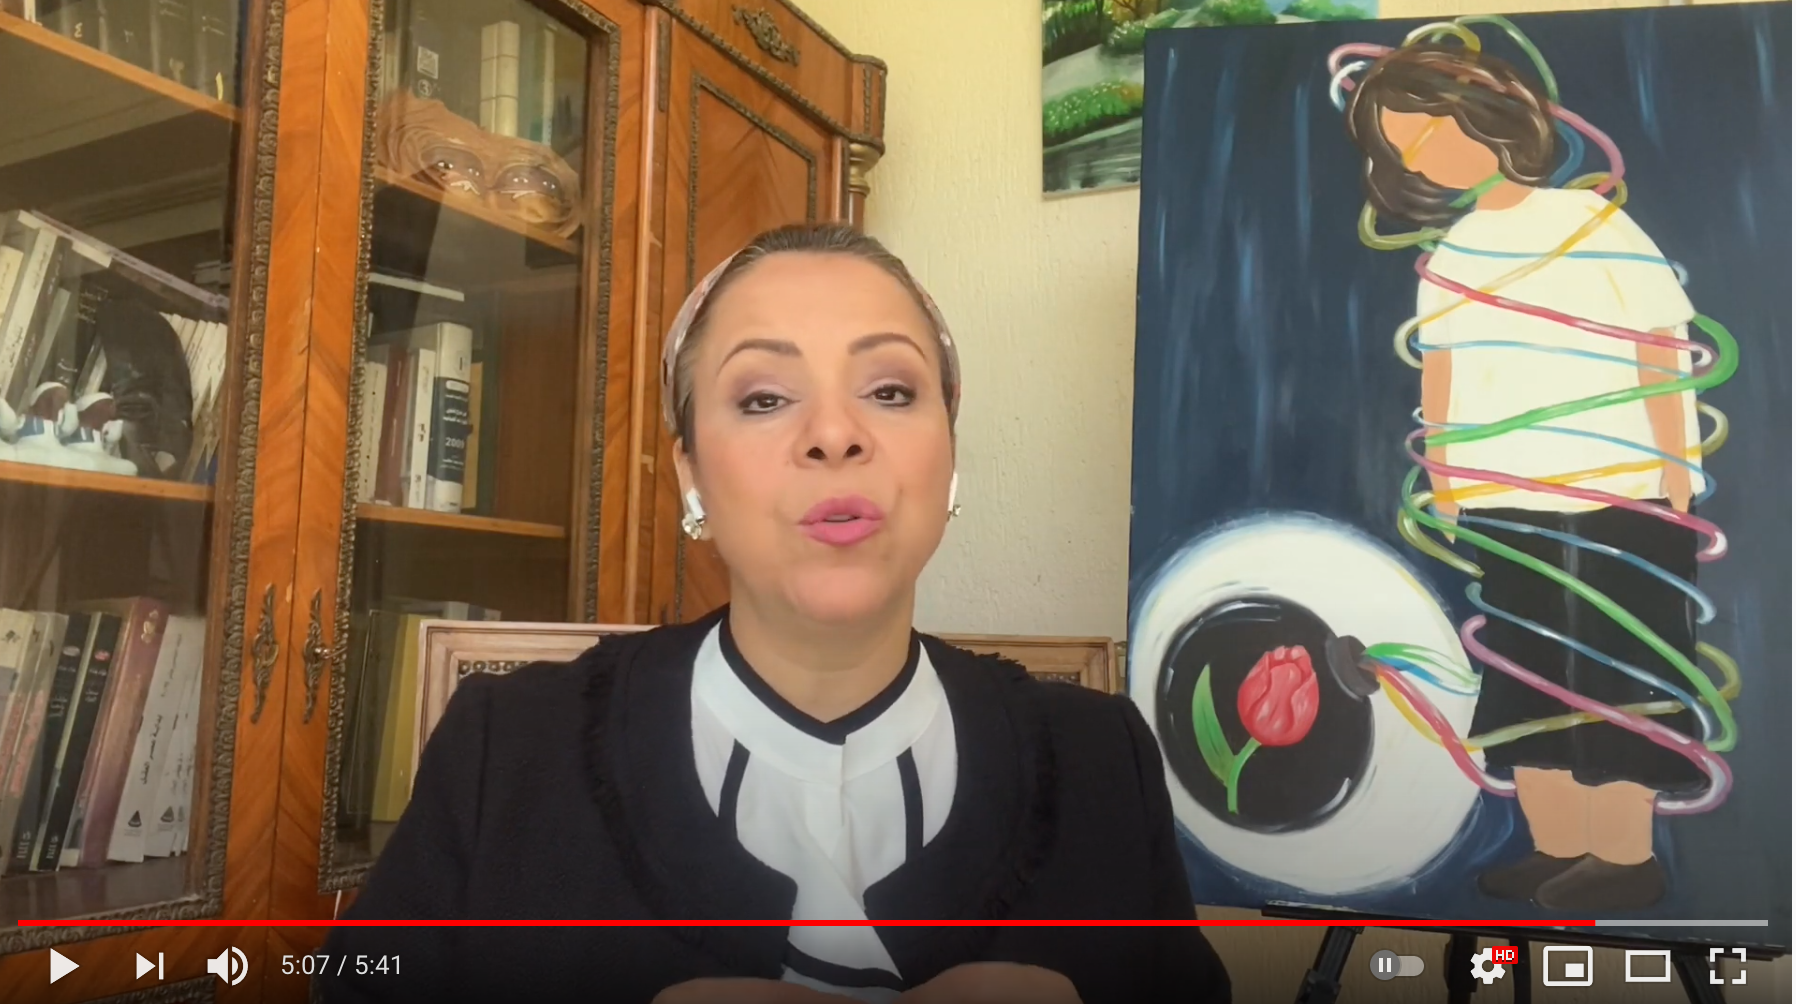
\includegraphics[width = 1\textwidth]{Recruit_Intervention/Nehad_sm.png}\captionsetup{font=small}
\caption{Our partner's social media videos were delivered from her home.  \href{https://youtu.be/ganxQqVxXng?t=306.}{ Link to a clip.}} 
 \end{figure} 
\end{column}
\begin{column}{0.5\textwidth}
\begin{figure}\onslide<1-> 
\includegraphics[width = 1\textwidth]{Recruit_Intervention/Nehad_TV.png}\captionsetup{font=small}
\caption{Our partner's TV show was more highly produced. \href{https://youtu.be/6ERGJkAUal4?t=557}{Link to a clip.}} 
 \end{figure} 
\end{column}
\end{columns}

\end{frame}

\begin{frame}{Treatment Take Up: Webpages Visited}
Aggregate website visits and YouTube views suggested moderate uptake, with the mean website visitor watching 2.6 videos.
\begin{figure}[H]
    \centering
    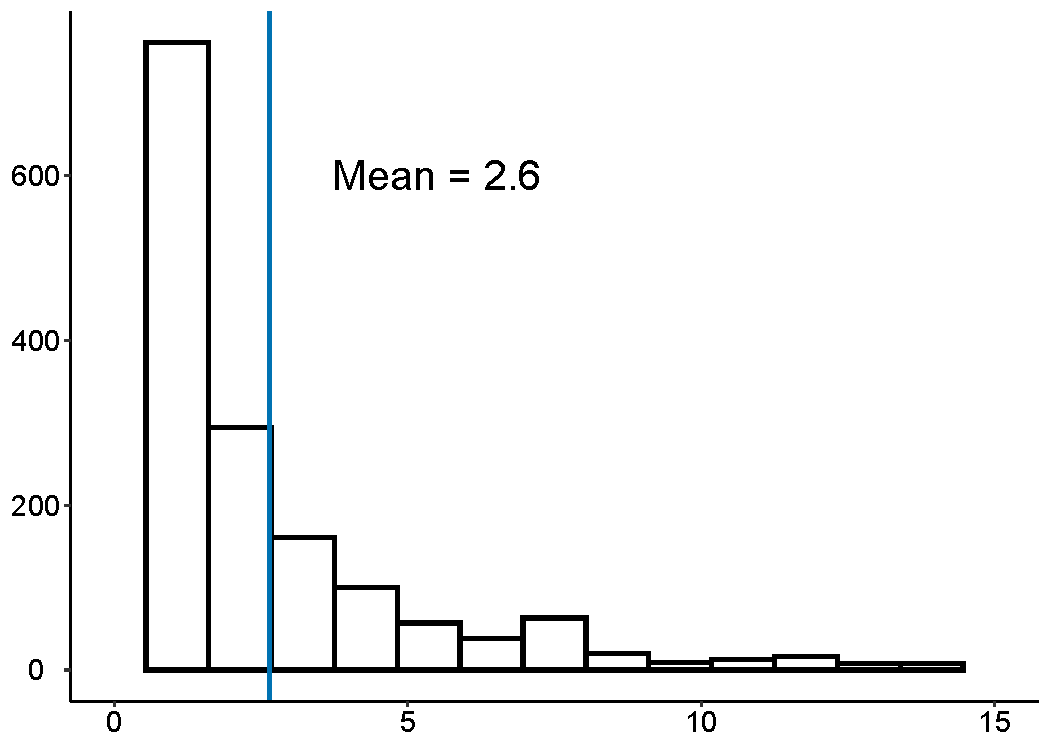
\includegraphics[height=6cm,width=8cm\linewidth]{Figures/Other/pages_all.pdf} 
    \caption{\scriptsize Number of treatment web pages visited per web page user across all treatments} 
\end{figure}
\end{frame}

\begin{frame}{Relatively Inefficient Facebook Delivery}
For one treatment arm, we transitioned from using Facebook Custom Messages to WhatsApp. We analyze Facebook and WhatsApp one-to-one messages jointly.
\begin{figure}[H]
%\caption{Video landing web page visits for Facebook and WhatsApp Individual treatment before and after participants assigned to the Facebook treatment were shifted to the WhatsApp Individual treatment} 
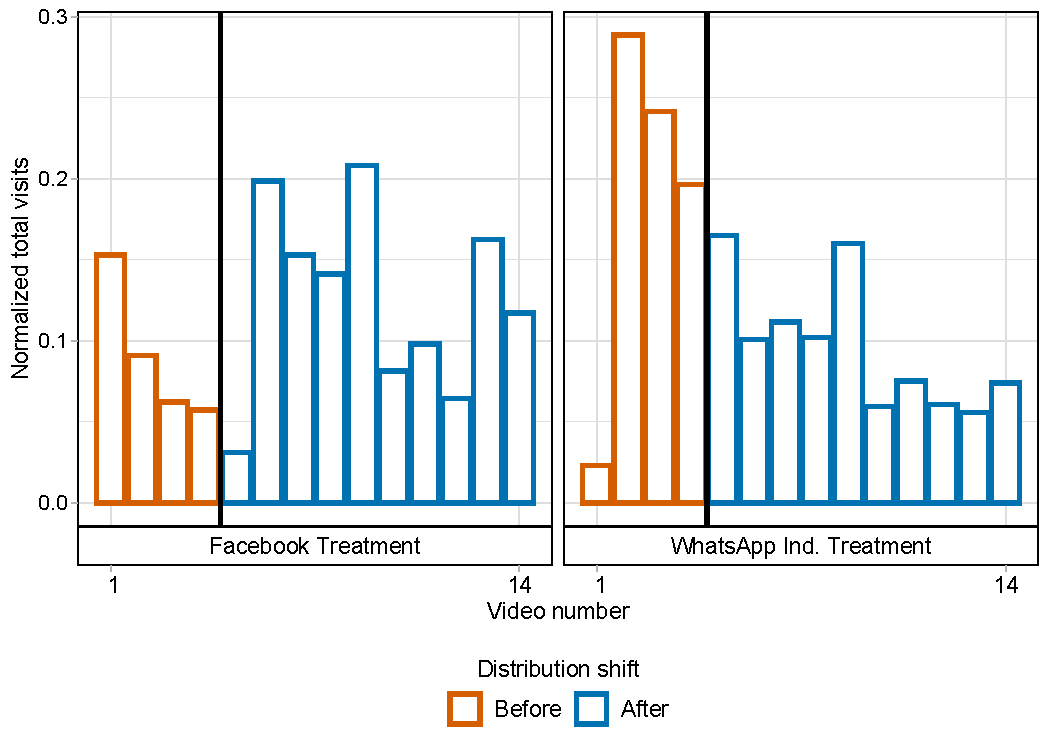
\includegraphics[width=0.8\textwidth]{Figures/Other/dist_change.pdf}
\captionsetup{width=.85\linewidth}
\label{fig:fb_shifts}
\end{figure}
\end{frame}



% \begin{frame}{Empirical Strategy}
% \begin{itemize}
%     \item We estimate WGLS regression, with weights corresponding to inverse probability of treatment assignment, with block randomization fixed effects
%     \item Our primary estimates are for WhatsApp and Facebook Individual, WhatsApp Group and TV
%     \begin{itemize}
        
%     \end{itemize}
% \end{itemize}
    
% \end{frame}

\section{Preliminary Results}
\begin{frame}{FS Results: Individuals in treatment arms viewed content and increased knowledge of resources}
\Wider[5em]{
\begin{figure}[H]
    \centering
   % \caption{Treatment effects for first stage TV, first stage Facebook and WhatsApp, and reduced form on knowledge}
    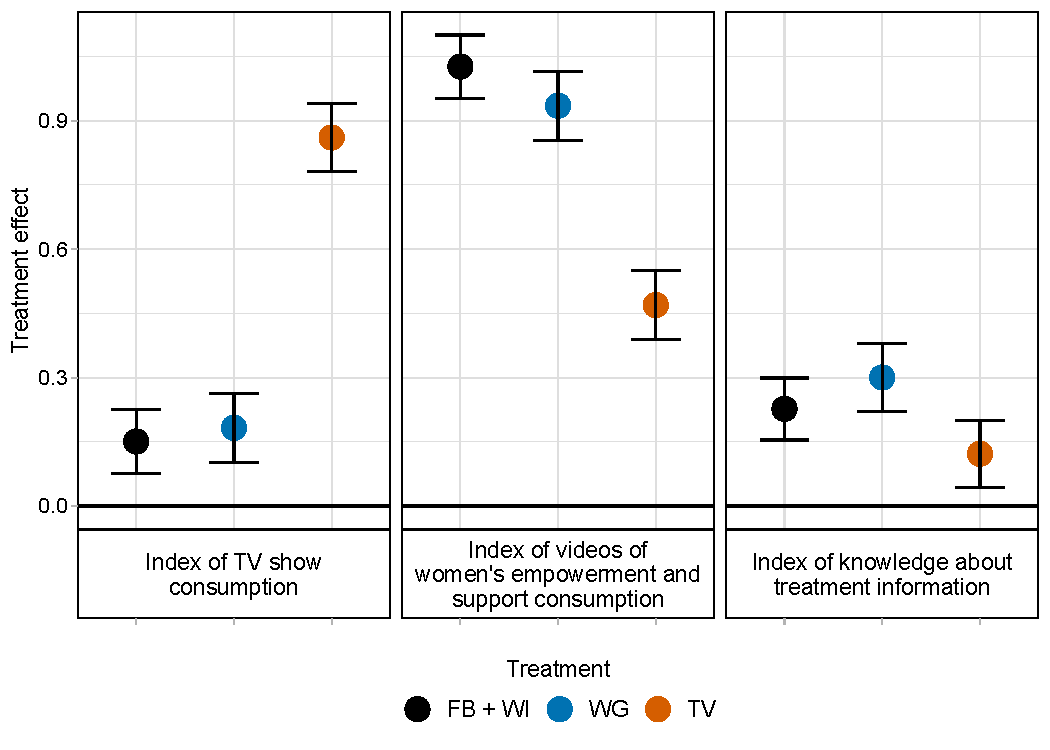
\includegraphics[width=0.6\textwidth, clip=true, trim = 0 13 0 5]{Figures/RF-FS/Figure2.pdf}
   % \captionsetup{width=1\linewidth}
%    \caption*{\footnotesize Treatment effects for first stage TV, first stage Facebook and WhatsApp, and reduced form on knowledge. Boxes represent separate WGLS regressions of dependent variable. Regressions using inverse probability weighting and block fixed effects (95\% confidence interval).}
\end{figure} 
\small
\begin{itemize}
    \item *Boxes display 95\% Confidence Interval from separate WGLS regressions of dependent variable, with inverse probability weighting and block fixed effects. All dependent variables are indices of battery of questions. 
    \item Example First Stage Measurement: Over the past two months, did you receive any videos on WhatsApp or Facebook related to women's empowerment in Egypt?
\end{itemize}
}
\end{frame}

\begin{frame}{FS Results: Individuals in treatment arms viewed content and increased knowledge of resources}
\Wider[5em]{
\begin{figure}[H]
    \centering
   % \caption{Treatment effects for first stage TV, first stage Facebook and WhatsApp, and reduced form on knowledge}
    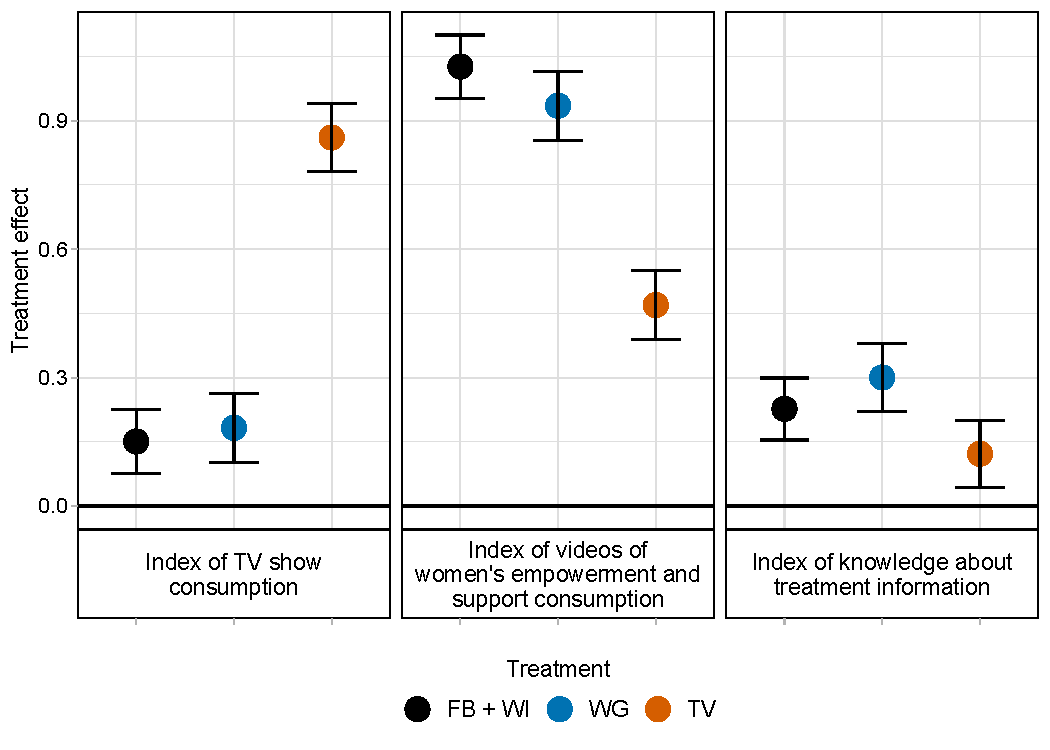
\includegraphics[width=0.6\textwidth, clip=true, trim = 0 13 0 5]{Figures/RF-FS/Figure2.pdf}
   % \captionsetup{width=1\linewidth}
%    \caption*{\footnotesize Treatment effects for first stage TV, first stage Facebook and WhatsApp, and reduced form on knowledge. Boxes represent separate WGLS regressions of dependent variable. Regressions using inverse probability weighting and block fixed effects (95\% confidence interval).}
\end{figure} 
\small
\begin{itemize}
    \item Example Knowledge Question: Which organizations do you know that support and advise women affected by domestic violence, or who face sexual harassment or assault? List up to five options. 
\end{itemize}
}
\end{frame}


\begin{frame}{RF Results: Intervention had no impact on attitudes}
\Wider[5em]{
\begin{figure}[H]
    \centering
    %\caption{Treatment effects on attitudes}
    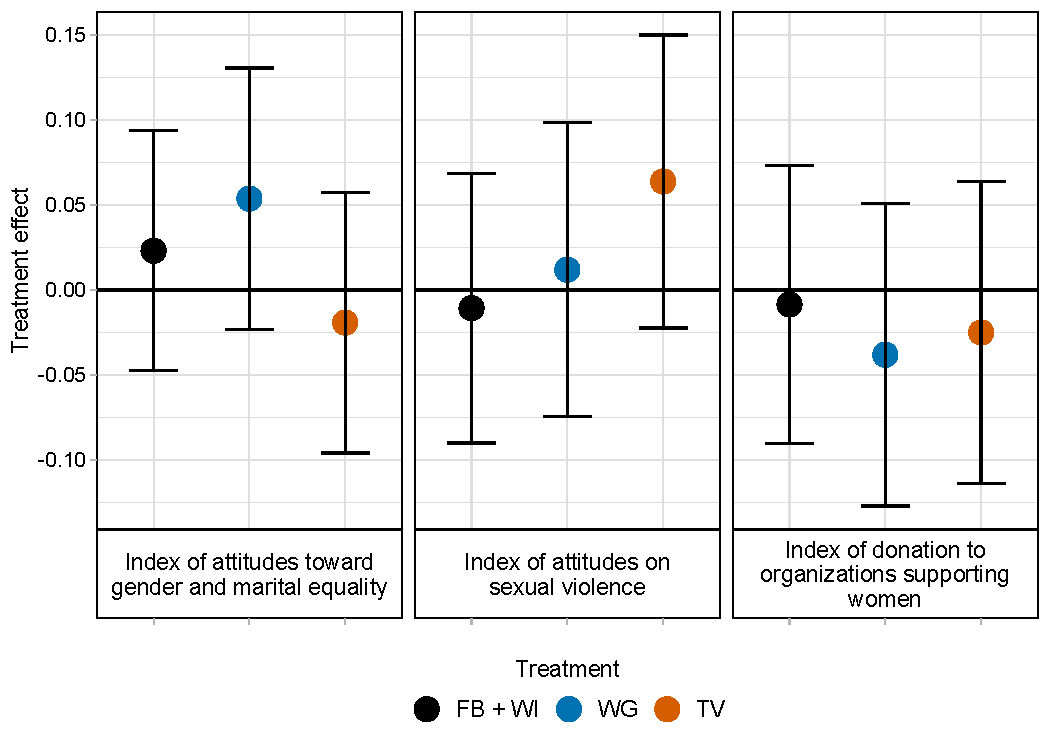
\includegraphics[width=0.6\textwidth, clip=true, trim = 0 13 0 5]
    {Figures/RF-FS/Figure3.pdf}
      %  \captionsetup{width=.75\linewidth}
   % \caption*{\footnotesize Treatment effects on attitudes. Sample questions: DV: Husbands are sometimes justified in yelling at their wives (e.g., when the wife disobeys them). Sexual violence: If a child in your family tells you that a relative you trust very much has sexually harassed them, you should take them seriously.}%\footnotesize \texit{Notes:} Each box is from a separate WGLS regression where the labels represent the corresponding dependent variable (weights are in the inverse probability of treatment assignment), including randomization block fixed effects (95\% confidence interval).}
\end{figure}
\small
\begin{itemize}
    \item Sample Domestic Violence Attitude: Husbands are sometimes justified in yelling at their wives (e.g., when the wife disobeys them). 
    \item Sample Sexual Violence Attitude: If a child in your family tells you that a relative you trust very much has sexually harassed them, you should take them seriously.
\end{itemize}}
\end{frame}


\begin{frame}{RF Results: Intervention shaped hypothetical behavior and use of resources}
\Wider[4em]{
    \begin{figure}[H]
    \centering
   % \caption{Treatment effects on hypothetical and reported behavior}
    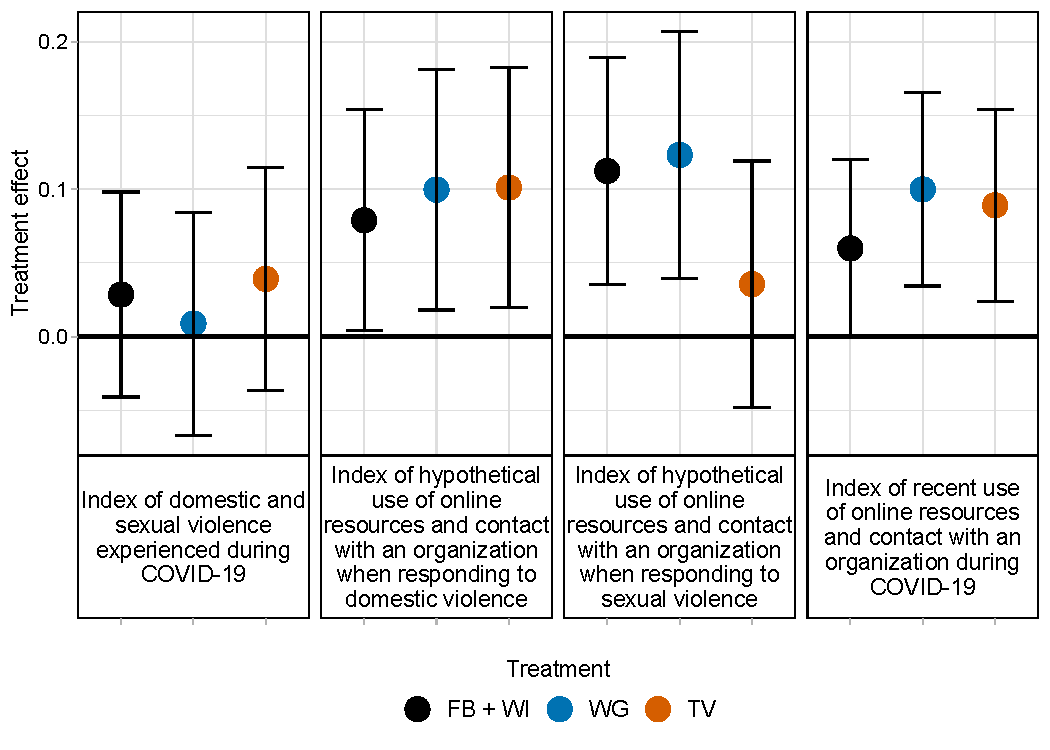
\includegraphics[width=0.6\textwidth, clip=true, trim = 0 13 0 5]{Figures/RF-FS/Figure4.pdf}
    \captionsetup{width=.75\linewidth}
   % \caption*{\footnotesize Treatment effects on hypothetical and reported behaviors of  looking for online resources or an organization. \\}
\end{figure}
\small 
\begin{itemize}
    \item Sample Hypothetical Behavior: Suppose that a friend tells you that she has been affected by domestic violence and asks you for your advice. How likely would you be to recommend her to: Contact an organization that supports and advises women affected by domestic violence?
\end{itemize}}
\end{frame}

\begin{frame}{RF Results: Intervention shaped hypothetical behavior and use of resources}
\Wider[4em]{
    \begin{figure}[H]
    \centering
   % \caption{Treatment effects on hypothetical and reported behavior}
    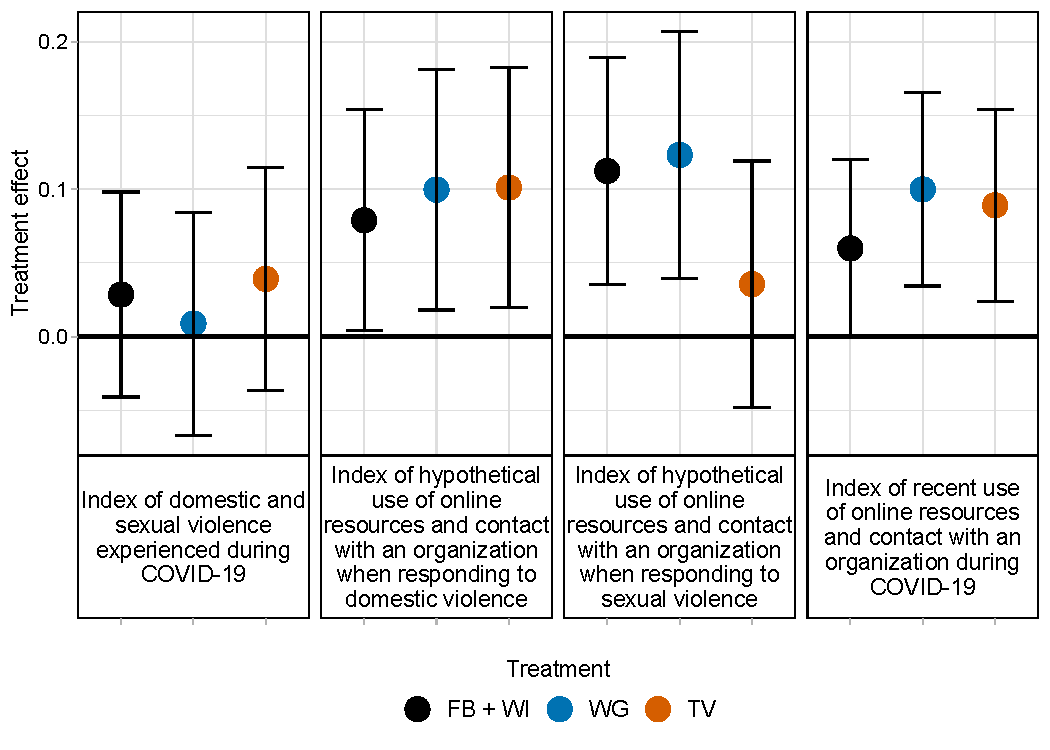
\includegraphics[width=0.6\textwidth, clip=true, trim = 0 13 0 5]{Figures/RF-FS/Figure4.pdf}
    \captionsetup{width=.75\linewidth}
   % \caption*{\footnotesize Treatment effects on hypothetical and reported behaviors of  looking for online resources or an organization. \\}
\end{figure}
\small
\begin{itemize}
    \item Sample Recent Behavior: Now DURING the COVID-19 pandemic, in the past month have you ever looked for or accessed online resources for women affected by domestic violence, or who faced sexual harassment or assault?
\end{itemize}}
\end{frame}


\begin{frame}{RF Results: Intervention positively shaped future outlook}
\Wider[4em]{
    \begin{figure}[H]
    \centering
    %\caption{Treatment effects on future outlook}
    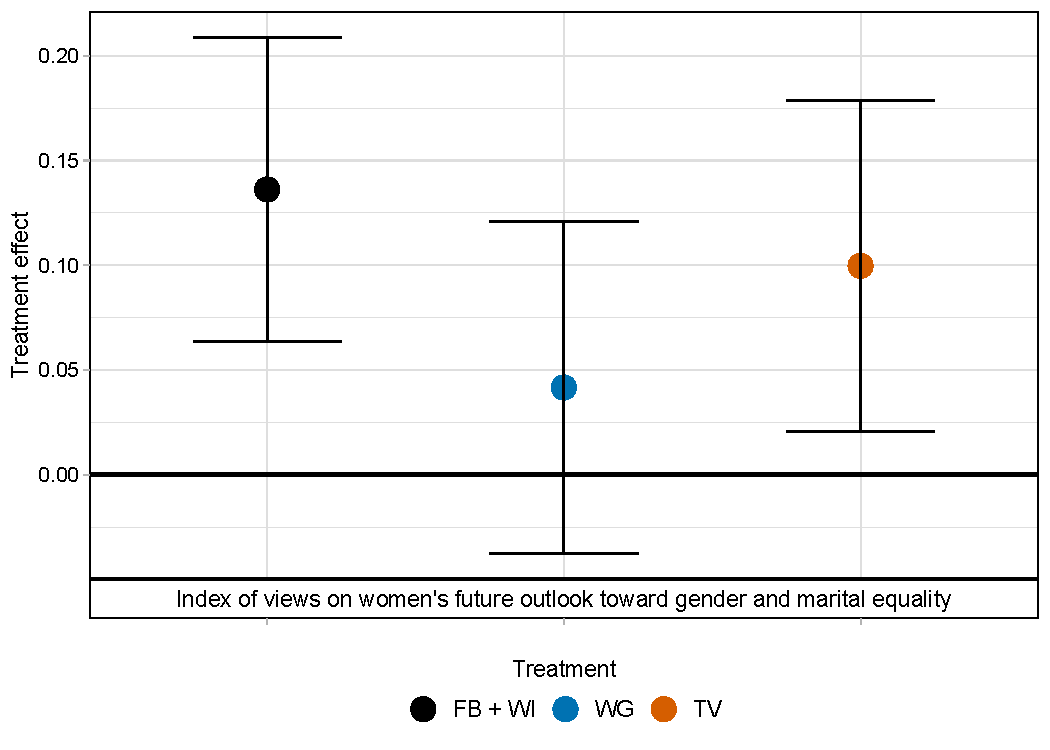
\includegraphics[width=0.6\textwidth, clip=true, trim = 0 13 0 5]{Figures/RF-FS/Figure5.pdf}
      %  \captionsetup{width=.75\linewidth}
    %\caption*{\footnotesize Treatment effects on future outlook.} %\texit{Notes:} Each box is from a separate WGLS regression where the labels represent the corresponding dependent variable (weights are in the inverse probability of treatment assignment), including randomization block fixed effects (95\% confidence interval).}
\end{figure}
\small
\begin{itemize}
    \item Future Outlook: In the future, women will have an equal say with their husbands in all decisions concerning the family.
    \item Future Outlook: In the future, men and women in Egypt will have more equal legal rights, access to education, and economic opportunities.
\end{itemize}}
\end{frame}


\section{Discussion and Contributions}
\begin{frame}{Discussion and Contributions}
\begin{itemize}
    \onslide<1-> \item Strong first stage suggests utility of social media as delivery method for edutainment interventions (esp. amid COVID-19), alongside continued role of formal/traditional media in shaping attitudes (Oster 2009, La Ferrara 2009).  \vspace{2mm}
    \onslide<2-> \item Behavioral shift despite limited or no attitudinal shifts in line with other recent experimental findings on GBV and IPV (Green et. al. 2020; Cooper et. al. 2020), deference to authority (Paluck \& Green 2009), reporting corruption (Blair et. al. 2019), prejudice reduction (Mousa 2020). \vspace{2mm}
   \onslide<3->  \item Limited difference between individual and community distribution channels could be due to absence of quality conversation or coordination in groups, especially online (Chwe 1998, Arias 2019). \vspace{2mm}
\end{itemize}
    
\end{frame}

\section{Appendix}
\begin{frame}{Appendix: Comparison of Attitudes and Behavior with Nationally Representative Survey}
\begin{figure}[H]
\caption{Comparison of Attitudes and Behavior with general (Arab Barometer) population \\}
   \begin{minipage}{0.8\textwidth} 
\begin{subfigure}{0.5\textwidth}
  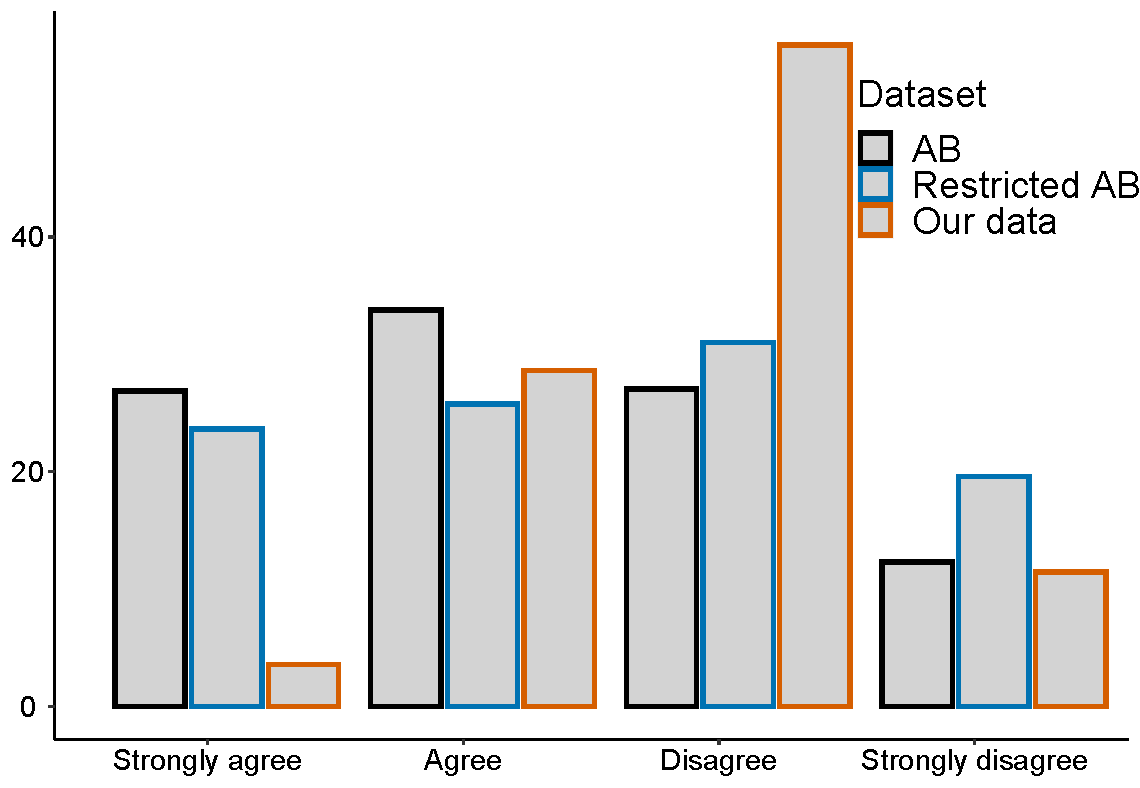
\includegraphics[height=3cm,width=4cm\linewidth]{Figures/AB/grey_solid/husb_fs.pdf} 
    \caption{Husband final say} 
    \label{} 
\end{subfigure}\hfil
\begin{subfigure}{0.5\textwidth}
  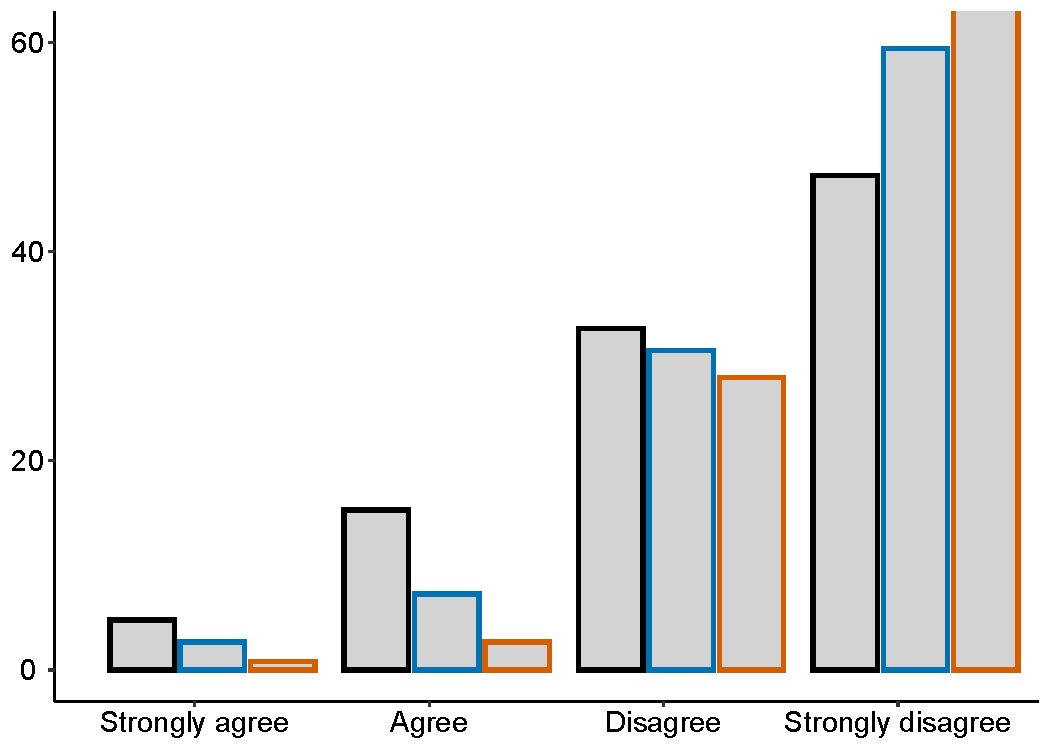
\includegraphics[height=3cm,width=4cm\linewidth]{Figures/AB/grey_solid/prio_educ.pdf} 
    \caption{Prioritize education of men} 
    \label{} 
\end{subfigure}\hfil
\begin{subfigure}{0.5\textwidth}
  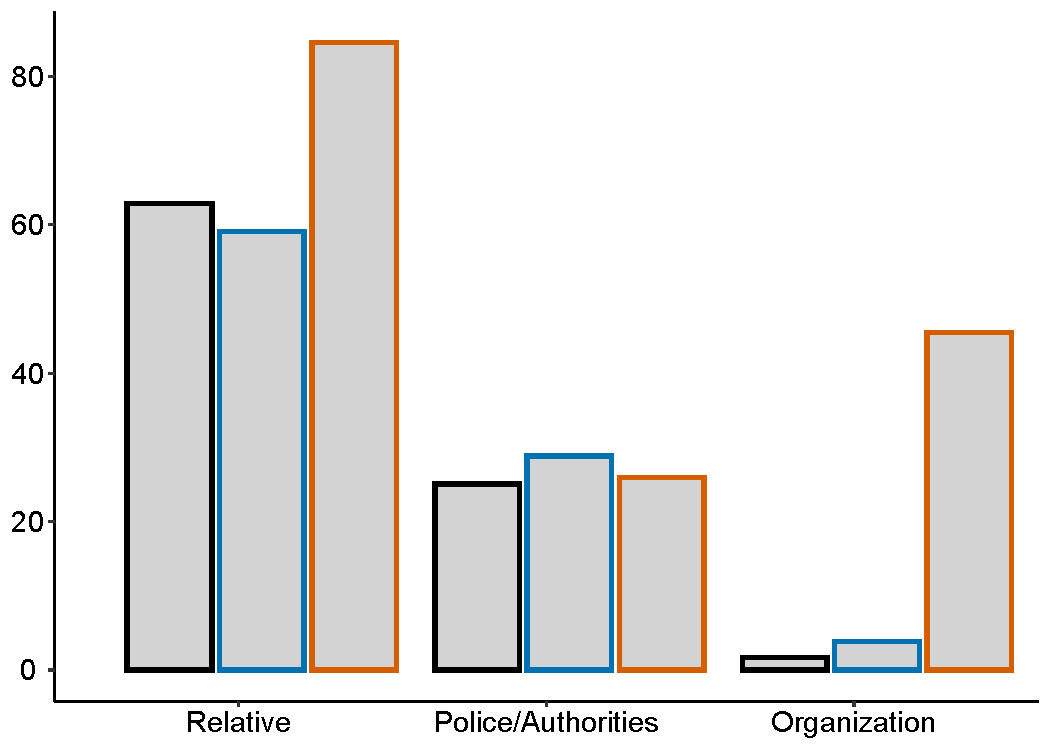
\includegraphics[height=3cm,width=4cm\linewidth]{Figures/AB/grey_solid/support.pdf} 
    \caption{Support Source in DV Experience/Scenario*} 
    \label{} 
    \end{subfigure}\hfil
    \begin{subfigure}{0.5\textwidth}
    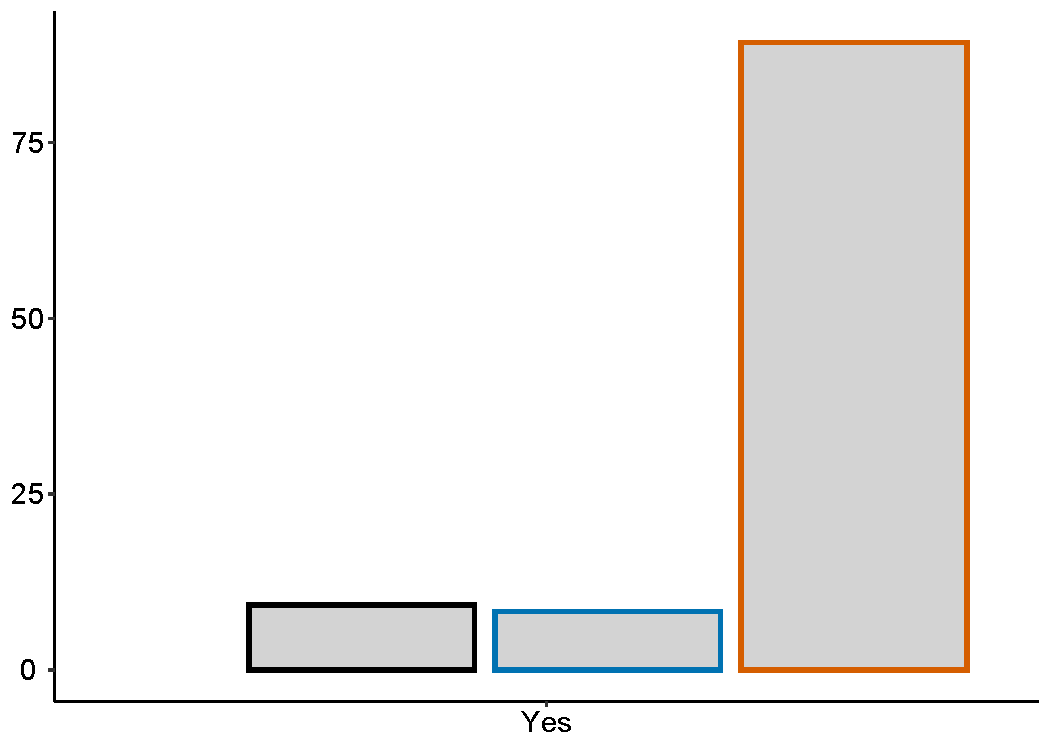
\includegraphics[height=3cm,width=4cm\linewidth]{Figures/AB/grey_solid/violence.pdf} 
    \caption{Experienced violence*} 
    \label{} 
  \end{subfigure} 
%\floatfoot{\footnotesize 
 %   \texit{Notes:} \textsuperscript{1}The “support from” variable is different in both surveys: in the AB survey, they asked how likely a family member who was physically abused by another relative be able to receive assistance from one of the actors, and we asked how likely you would be to recommend your friend to talk/report to one of the actors. \textsuperscript{2}The “Experienced violence” variable is different in both surveys: in the AB survey they asked if in the last twelve months a female member of your household experienced being physically abused by another member of your family, and we asked if in the month before the COVID-19 pandemic, how frequently did you hear of someone being hit by a man, and we took as valid all answers that specify at least once.}
\end{minipage}
  \label{}
\end{figure}
    
\end{frame}

\begin{frame}{Appendix: Video Content}
\Wider[5em]{
    \begin{table}[ht]
\centering
\scalebox{0.6}{
\begin{tabular}{|p{6cm}|p{1.5cm}|p{2cm}|p{1.5cm}|p{1.5cm}|p{1.5cm}|p{1.5cm}|p{1.5cm}|}
  \hline
Title & Date & YT Views & Web Visits & YT Total (Hours) & Web Total (Hours) & YT Avg. View & Web Avg. Visit \\ 
  \hline
What is sexual harassment and what is its penalty?  &  Jul 24  & 535  & 682 & 22.80 & 40.26 &  0:02:33  & 0:03:33 \\ \hline
  Sexual harassment of children and how to protect them?   &  Jul 31  & 391  & 493 & 24.42 & 40.66 &  0:03:44  & 0:04:57 \\ \hline
  Are womens clothes the cause of sexual harassment?  &  Aug 3  & 324  & 372 & 15.26 & 21.59 &  0:02:49  & 0:03:29 \\ \hline
  FGC and how to stop it?  &  Aug 7  & 268  & 286 & 18.19 & 22.16 &  0:04:04  & 0:04:39 \\ \hline
  Impact of COVID-19 on increasing domestic violence  &  Aug 11  & 212  & 235 & 9.84 & 17.85 &  0:02:47  & 0:04:33 \\ \hline
  Rape crimes and how to fight them and COVID-19  &  Aug 14  & 207  & 226 & 9.97 & 12.02 &  0:02:53  & 0:03:11 \\ \hline
  The difference between divorce and Khul and when to choose either?  &  Aug 17  & 268  & 230 & 15.09 & 18.55 &  0:03:22   & 0:04:50 \\ \hline
  The importance of work and how to balance between work and home?   &  Aug 21  & 281  & 268 & 18.03 & 21.35 &  0:03:51  & 0:04:47 \\ \hline
  The negative effects of Covid-19 on women’s work  &  Aug 25  & 107  &  96 & 5.22 & 4.60 &  0:02:55   & 0:02:52 \\ \hline
  How to deal with workplace harassment?  &  Aug 26  & 175  & 143 & 9.83 & 10.84 &  0:03:22   & 0:04:33 \\ \hline
  How to act if you saw someone harassing a colleague at work?  &  Aug 28  & 146  & 110 & 7.10 & 7.86 &  0:02:55   & 0:04:17 \\ \hline
  Dealing with workplace harassment for new employees  &  Sep 7  & 172  & 146 & 7.84 & 10.55 &  0:02:44  & 0:04:20 \\ \hline
  How can men stand against violence against women?   &  Sep 9  & 184  & 184 & 7.84 & 21.02 &  0:02:33   & 0:06:51 \\ \hline
   Totals  &  & 3270 & 3471 & 13.19 & 19.18 & 0:02:59 & 0:04:22 \\
   \hline
\end{tabular}
}
\caption{Website and YouTube analytics show that earlier videos received higher numbers of visitors and views. The website analytics report higher numbers because they measure individual visits and total duration on the site, whereas YouTube measures time spent viewing the content.} 
\label{table:youtube_views}
\end{table}}
\end{frame}


\begin{frame}{Sample Reporting Text}
\begin{center}
\say{...If you see [these types of sexual harassment] happening to anyone, we need to stop it in its entirety. If you are in a position where you see something happening in front of you and you need to consult with someone, talk to us at the Egyptian Center for Women’s Rights on the hotline, 19576. There is an effective team that will help you with what to do in positions like this one. There is also the Egyptian Council for Women, 15115, that can also help you with how to act in these situations.}
\end{center}

    
\end{frame}
\end{document}